\documentclass[10pt]{beamer}

%\documentclass[12pt]{article}

\usepackage{tikz}
\usepackage{mathtools}
\usepackage{xcolor}
\usetikzlibrary{arrows,automata,positioning}
\usetikzlibrary{arrows.meta,positioning}
\definecolor{darkgreen}{rgb}{0.0, 0.5, 0.0}
%\begin{document}

% images:
% \maxIndependentSet
% \maxFlow
% \mvcInsufficient
% \mvcSufficient
% \chromaticNumber
% \exampleLPConstraints
% \primalSimplexExample
% \milpExample


% adapted from https://tex.stackexchange.com/questions/341949/how-to-plot-a-network-flow-with-tikz
\newcommand{\maxFlow}{
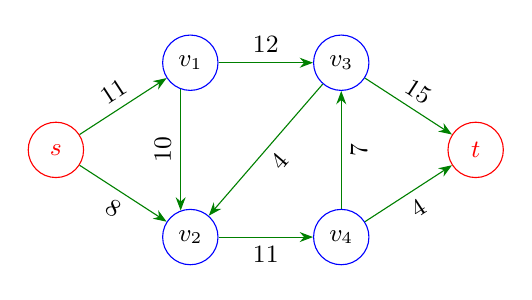
\begin{tikzpicture}[
      mycircle/.style={
         circle,
         draw=blue,
         text opacity=1,
         inner sep=0pt,
         minimum size=20pt,
         font=\small},
      myarrow/.style={-Stealth, draw=darkgreen},
      node distance=0.6cm and 1.2cm
      ]
      \node[mycircle, red] (c1) {$s$};
      \node[mycircle,below right=of c1] (c2) {$v_2$};
      \node[mycircle,right=of c2] (c3) {$v_4$};
      \node[mycircle,above right=of c1] (c4) {$v_1$};
      \node[mycircle,right=of c4] (c5) {$v_3$};
      \node[mycircle,below right=of c5, red] (c6) {$t$};

    \foreach \i/\j/\txt/\p in {% start node/end node/text/position
      c1/c2/8/below,
      c1/c4/11/above,
      c2/c3/11/below,
      c3/c6/4/below,
      c4/c5/12/above,
      c5/c6/15/above,
      c5/c2/4/below,
      c3/c5/7/below}
       \draw [myarrow] (\i) -- node[sloped,font=\small,\p] {\txt} (\j);


     % draw this outside loop to get proper orientation of 10
     \draw [myarrow] (c4.250) -- node[sloped,font=\small,above,rotate=180] {10} (c2.110);
¸\end{tikzpicture}
}

\newcommand{\mvcInsufficient}{
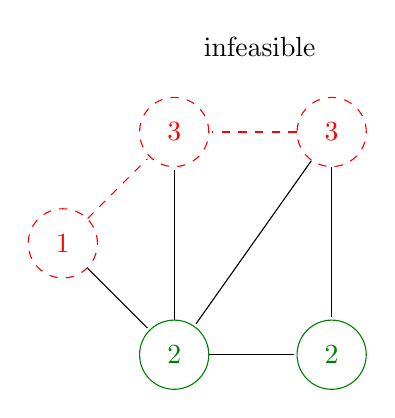
\begin{tikzpicture}[shorten >=1pt,node distance=2cm,on grid,auto]

\node[state,red, dashed] (x1)                      	 {$1$};
\node[state, darkgreen] (x2)[below right of=x1]	 {$2$};
\node[state, red, dashed] (x3)[above right of=x1]	 {$3$};
\node[state, darkgreen] (x4)[right of=x2]		 {$2$};
\node[state, red, dashed] (x5)[right of=x3]	 	 {$3$};

\path[-]
    (x1)	edge node {} (x2)
    (x2)	edge node {} (x4)
    		edge node {} (x3)
    (x5)	edge node {} (x4)
    		edge node {} (x2);

\path[-, dashed, red]
    (x1)		edge node [dashed, red] {} (x3)
    (x5)	edge node [dashed, red] {} (x3);
    
\node[] at (2.5,2.5) {infeasible};
\end{tikzpicture}
}

\newcommand{\mvcSufficient}{
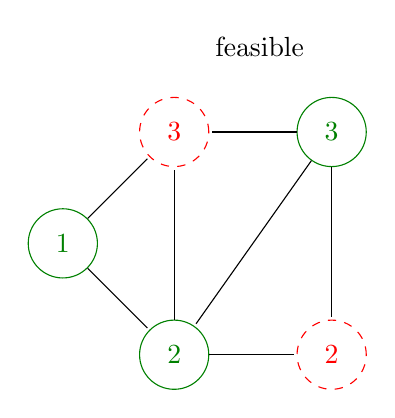
\begin{tikzpicture}[shorten >=1pt,node distance=2cm,on grid,auto]

\node[state,darkgreen]    (x1)                       {$1$};
\node[state, darkgreen]   (x2)[below right of=x1]	 {$2$};
\node[state, red, dashed] (x3)[above right of=x1]	 {$3$};
\node[state, red, dashed] (x4)[right of=x2]		     {$2$};
\node[state, darkgreen]   (x5)[right of=x3]	 	     {$3$};

\path[-]
    (x1)	edge node {} (x2)
    		edge node {} (x3)
    (x2)	edge node {} (x4)
    		edge node {} (x3)
    (x5)	edge node {} (x3)
    		edge node {} (x4)
    		edge node {} (x2);
    		
\node[] at (2.5,2.5) {feasible};
\end{tikzpicture}
}

\newcommand{\chromaticNumber}{
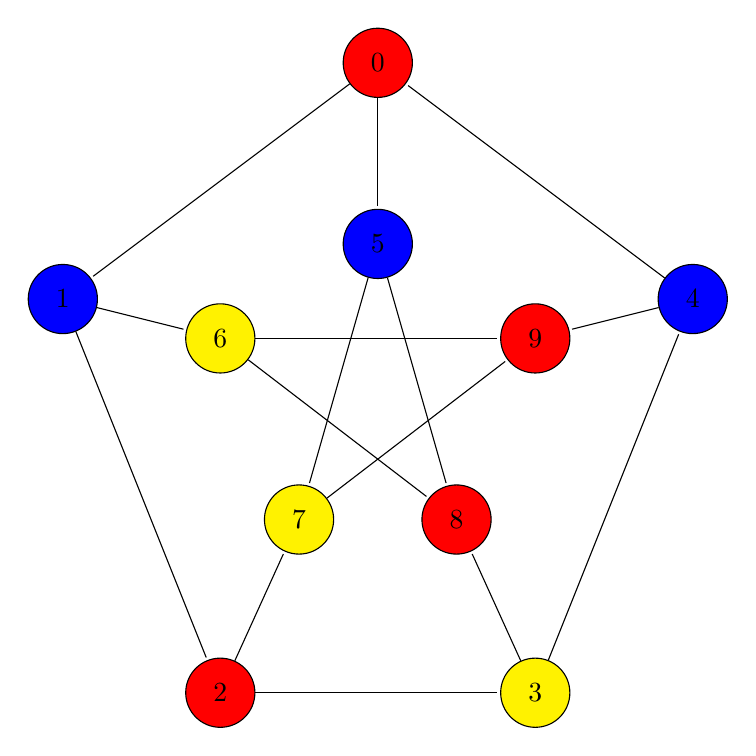
\begin{tikzpicture}[shorten >=1pt,node distance=2cm,on grid,auto, draw=black]

\node[state,fill=red]    (x0) at (5,9)                     {$0$};
\node[state,fill=blue]    (x1) at (1,6)                    {$1$};
\node[state,fill=red]    (x2) at (3,1)                     {$2$};
\node[state,fill=yellow]    (x3) at (7,1)               {$3$};
\node[state,fill=blue]    (x4) at (9,6)                    {$4$};

\node[state,fill=blue]    (x5)  at (5,6.7)                 {$5$};
\node[state,fill=yellow]    (x6)  at (3,5.5)            {$6$};
\node[state,fill=yellow]    (x7)  at (4,3.2)            {$7$};
\node[state,fill=red]    (x8)  at (6,3.2)                  {$8$};
\node[state,fill=red]    (x9) at (7,5.5)                   {$9$};

\foreach \f/\t in {% start node/end node
	 x0/x5,
	 x1/x6,
	 x2/x7,
	 x3/x8,
	 x4/x9,
	 x0/x1,
	 x1/x2,
	 x2/x3,
	 x3/x4,
	 x4/x0,
	 x5/x7,
	 x5/x8,
	 x6/x8,
	 x6/x9,
	 x7/x9}
	\path[-, draw=black]  (\f) edge node {} (\t);

\end{tikzpicture}
}

\newcommand{\maxIndependentSet}{
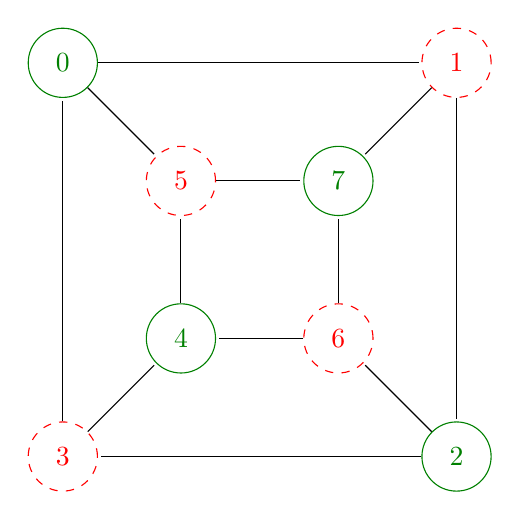
\begin{tikzpicture}[shorten >=1pt,node distance=2cm,on grid,auto, draw=black]

\node[state,darkgreen]    	(x0) at (0,5)               {$0$};
\node[state,red, dashed]    	(x1) at (5,5)               {$1$};
\node[state,darkgreen]    	(x2) at (5,0)               {$2$};
\node[state,red, dashed]  (x3) at (0,0)               {$3$};


\node[state,darkgreen]    	(x4) at (1.5,1.5)            {$4$};
\node[state,red, dashed]    	(x5) at (1.5,3.5)            {$5$};
\node[state,red, dashed]    	(x6) at (3.5,1.5)            {$6$};
\node[state,darkgreen]  (x7) at (3.5,3.5)            {$7$};



\foreach \f/\t in {% start node/end node
	 x0/x1,
	 x1/x2,
	 x2/x3,
	 x3/x0,
	 x4/x5,
	 x5/x7,
	 x6/x7,
	 x6/x4,
	 x3/x4,
	 x0/x5,
	 x1/x7,
	 x2/x6}
	\path[-]  (\f) edge node {} (\t);

\end{tikzpicture}
}


\newcommand{\drawLine}[4]{
\draw [darkgreen, line width=0.5mm] (#1,#2)--(#3,#4);
}
\newcommand{\drawDashedLine}[4]{
\draw [red, line width=0.2mm, dashed] (#1,#2)--(#3,#4);
}

% parts of a tikz picture for an example LP
\newcommand{\exampleLP}{
\draw [help lines, gray, line width=0.02mm] (0,0) grid (5,4);

% Euclidean
\draw [->](0,0)--(0,4) node[right]{$y$};
\draw [->](0,0)--(5,0) node[right]{$x$};

% draw ticks and its labels
\foreach \x/\xtext in {1/1, 2/2, 3/3, 4/4, 5/5}
{\draw (\x cm,1pt ) -- (\x cm,-1pt ) node[anchor=north] {$\xtext$};}
\foreach \y/\ytext in {1/1, 2/2, 3/3, 4/4}
{\draw (1pt,\y cm) -- (-1pt ,\y cm) node[anchor=east] {$\ytext$};}

\drawLine{2}{3}{3}{3}
\drawDashedLine{3}{3}{5}{3}
\drawDashedLine{0}{3}{2}{3}

\drawLine{0}{2}{2}{3}
\drawDashedLine{2}{3}{4}{4}

\drawLine{0}{0}{0}{2}
\drawDashedLine{0}{2}{0}{4}

\drawLine{0}{0}{5}{0}

\drawLine{5}{0}{4}{2}
\drawDashedLine{4}{2}{3}{4}

\drawLine{4}{2}{3}{3}
\drawDashedLine{4}{2}{5}{1}
\drawDashedLine{2}{4}{3}{3}

% objective function
\draw [cyan, line width=0.5mm] (1,4)--(5,2);
\coordinate[label = above right:\textcolor{cyan}{max}]() at (1.625,3.625);
\draw [dashed,->,>=stealth, line width=0.5mm, cyan] (1.375,3.5) -- (1.5,3.75);
\draw [dashed,->,>=stealth, line width=0.5mm, cyan] (4.375,2) -- (4.5,2.25);
}

% MILP example
\newcommand{\milpExample}{
\begin{tikzpicture}[scale=1]
\exampleLP

\foreach \x/\y in {0/0, 1/0, 2/0, 3/0, 4/0, 5/0, 0/1, 1/1, 2/1, 3/1, 4/1, 0/2, 1/2, 2/2, 3/2, 4/2, 2/3, 3/3}
{\node at (\x,\y) [circle,fill, blue,inner sep=1.5pt]{}; }
\end{tikzpicture}
}

\newcommand{\drawArrowLine}[4]{
\draw [blue, line width=0.5mm, -stealth] (#1,#2)--(#3,#4);
}
\newcommand{\primalSimplexExample}{
\begin{tikzpicture}[scale=1,]
\exampleLP


\foreach \i/\x/\y in {1/0/0, 2/5/0, 3/3.25/1.25, 4/2.25/2.25}
{\coordinate[label = above right:$(\i)$]() at (\x,\y);}

\foreach \i/\x/\y in {1/0/0, 2/5/0, 3/4/2, 4/3/3}
{\node at (\x,\y) [circle,fill, black,inner sep=2pt](x){};}
\drawArrowLine{0}{0}{5}{0}
\drawArrowLine{5}{0}{4}{2}
\drawArrowLine{4}{2}{3}{3}
\end{tikzpicture}
}

\newcommand{\exampleLPConstraints}{
\begin{tikzpicture}[scale=1]
\exampleLP


\foreach \i/\x/\y in {1/0/0.5, 2/2/0, 3/1/2, 4/2.1/2.3, 5/2.9/1.9, 6/3.8/0.4}
{\coordinate[label = above right:\rProp{\i}]() at (\x,\y); }

\end{tikzpicture}
}

%\end{document}
\usetheme[progressbar=frametitle]{metropolis}
\usepackage{appendixnumberbeamer}
\usepackage{amsmath}
\usepackage{amssymb}
\usepackage{booktabs}
\usepackage[scale=2]{ccicons}
\usepackage{pgfplots}
\usepgfplotslibrary{dateplot}
\usepackage{wrapfig}

\usepackage{xspace}
\newcommand{\themename}{\textbf{\textsc{metropolis}}\xspace}
\setbeamercolor{frametitle}{bg=mpigreen}
\newcommand{\primaryColor}[1]{\textcolor{mpigreen}{#1}}
\newcommand{\primaryColorB}[1]{\textcolor{mpigreen}{\textbf{#1}}}
\newcommand{\q}[1]{``#1``}
\title{Introduction to mathematical programming}

\author{Julien Meier}
\newcommand{\curlO}{\{\,\,}
\newcommand{\curlC}{\,\,\}}

\newcommand{\nphard}{$\mathcal{NP}$-hard\,}

\begin{document}


\maketitle

\begin{frame}{Damn, it is about mathematics?!}
Nope, it is not - at least not really if you're not delving into the theory.\\\,\\


This will be more about modelling of problems from practice and the theoretical basics.
\end{frame}


\begin{frame}{Why should we care?}
Because...
\begin{enumerate}
	\item we can easily \primaryColorB{solve difficult problems}
	\item it serves as a \primaryColorB{first approach}
	\item it might help \primaryColorB{approximating} problems
	\item \primaryColorB{Braun} loves it! (awesome for your PA)
	\item it is widely used in \primaryColorB{practice}
\end{enumerate}
\end{frame}


\begin{frame}{Agenda}
\begin{enumerate}
	\item Example problems
	\item Basics of modelling
	\item Applying the techniques
	\item Staying realistic
\end{enumerate}
\end{frame}

\begin{frame}{What can we model?}
A lot!\\\,\\

Let's look at some examples...
\end{frame}



\begin{frame}{Example: Maximum flow (\q{easy} problem)}
\primaryColorB{Problem:} Maximum flow\\
\primaryColorB{Goal:} How much flow can you push from node $s$ to node $t$ while complying with capacity constraints.\\

\begin{figure}
	\centering
	\scalebox{1.4}{\maxFlow}
	\caption{Example for maximum flow. Upper bound is 19 units due to the capacity constraints of the edges going into $t$.}
\end{figure}
\end{frame}

\begin{frame}{Example: Minimum Vertex Cover (\nphard)}
\primaryColorB{Problem:} Minimum Vertex Cover\\
\primaryColorB{Goal:} Find a subset of vertices that cover each edge while minimizing costs.\\

\begin{figure}
	\centering
\begin{tabular}{c c}
	\mvcSufficient
	\mvcInsufficient
\end{tabular}
	\caption{Example for minimum vertex cover. Numbers in nodes are associated costs. Dashed edges are not covered which renders the instance infeasible. All dashed nodes are not included in the subset.}
\end{figure}
\end{frame}


\begin{frame}{Example: Graph coloring (\nphard)}
\primaryColorB{Problem:} Graph coloring\\
\primaryColorB{Goal:} Color each node with adjacent nodes colored distinctly.\\

\begin{figure}
	\centering
	\scalebox{0.6}{\chromaticNumber}
	\caption{Example for graph coloring. Adjacent nodes are colored distinctly.}
\end{figure}
\end{frame}



\begin{frame}{Example: Maximum Independent Set (\nphard)}
\primaryColorB{Problem:} Maximum Independent Set\\
\primaryColorB{Goal:} Find a maximum subset of vertices that are not adjacent.\\

\begin{figure}
	\centering
	\scalebox{0.8}{\maxIndependentSet}
	\caption{Example for maximum independent set. Dashed edges are excluded from the set. Note that none of the vertices included are adjacent.}
\end{figure}
\end{frame}

\begin{frame}{Short \q{reminder} on what's \nphard}
A problem being \nphard\, means \\$\qquad$ \textit{\q{probably not solvable deterministically in sub-exponential time}}\\ $\rightarrow$ difficult problem...\\\,\\
More precisely, a problem $B$ is \nphard\, if you can reduce another \nphard problem $A$ to it. Basic idea: Solve $A$ by solving $B$.\\\,\\
Reduction: $A \rightarrow B$ (formulate problem $A$ as problem $B$, solve it, then derive knowledge from that)
\end{frame}


\begin{frame}{How do we model these problems?}
Well, that's easy!\\\,\\

Using:
\begin{enumerate}
	\item A bunch of \primaryColorB{variables}
	\item An \primaryColorB{objective function} we want to \textit{minimize}/\textit{maximize}
	\item A lot of \primaryColorB{constraints} in the form of \primaryColorB{inequalities}
\end{enumerate}

\end{frame}


\begin{frame}{Component 1: Variables}

Variables $x_1, ..., x_n$ can be defined to be constrained to:
\begin{enumerate}
	\item $x_i\in \mathbb{R}$
	\item $x_i\in \mathbb{Z}$ (makes it difficult)
\end{enumerate}
\,\\
Using a suited solver and the \q{program} we define, we can get the variables' optimal values.
\end{frame}

\begin{frame}{Component 2: Objective function (1)}

The solver is given an objective function that should be \textit{minimized}/\textit{maximized}.\\
Thus, the optimal value is a \textit{variable assignment} that has minimal/maximal value.\\

\end{frame}

\begin{frame}{Component 2: Objective function (2)}
How does it look like?\\

\begin{equation}
	max \curlO 2x_1 + 3x_2 - 4x_3\curlC
\end{equation}

Trivial! Why not set everything to either $\infty$ or $-\infty$?\\
In the real world, everything is constrained.\\\,\\

The objective function \primaryColorB{should} be linear.

\end{frame}


\begin{frame}{Component 2: Objective function (3)}

What could we minimize/maximize?\\
Examples:
\begin{itemize}
	\item Minimize the colors used in the coloring problem.
	\item Maximize the flow in the max flow problem.
	\item Minimize the cost in Minimum Vertex Cover.
	\item Maximize the cardinality of the Maximum Independent Set problem.
\end{itemize}

\end{frame}

\begin{frame}{Component 3: Constraints (1)}

Constraints are linear inequalities of the form:
\begin{equation}
	3x_2 - 4x_3 \leq 5
\end{equation}
\,\\
In general with $m$ inequalities and $n$ variables
\begin{equation}
	\sum\limits_{i=1}^{n} a_{j,i}\cdot x_i \leq b_j,\qquad j\in \curlO 1, ..., m \curlC
\end{equation}
with constants $a_{j,i} \in \mathbb{R}$, $b_j\in \mathbb{R}$ and decision variables $x_i$.
\end{frame}

\begin{frame}{Component 3: Constraints (2)}

What can we model using $\leq$-constraints?\\\,\\
Well, in the \q{easy} case (none of the variables is integral)
\begin{enumerate}
	\item $\geq$ by multiplying with $-1$.
	\item $a=b$ by splitting into $a\leq b$ and $a\geq b$.
\end{enumerate}


\end{frame}


\begin{frame}{Component 3: Constraints (3)}

We can define \q{binary} values as follows:\\
\begin{equation}
	0\leq x \leq 1, \qquad x\in \mathbb{Z}
\end{equation}

Using binary values we can create constraints of the form $a != b$.\\\,\\
We define $x \in \mathcal{B} = \curlO 0,1\curlC$ to indicate that $x\in \mathbb{Z}$ and $0\leq x\leq 1$.

\end{frame}


\begin{frame}{Putting it all together}
Let's solve the Maximum Independent Set problem using a MILP:\\


\begin{wrapfigure}{r}{0.5\textwidth}
  \scalebox{0.75}{\maxIndependentSet}
\end{wrapfigure}
\,\\\,\\
\primaryColorB{Variables}:\, $x_0, x_1, ..., x_7 \in \mathcal{B}$\\\,\\
\primaryColorB{Objective}: $max \curlO\sum\limits_{i=0}^{7} x_i\curlC$\\\,\\
\primaryColorB{Constraints}:\\
For every edge $e=\curlO i,j\curlC$, \\$\qquad$ we create a constraint:\\
	$\qquad x_i + x_j \leq 1$
\end{frame}


\begin{frame}{Demo (1)}

\begin{center}
	\Huge \primaryColorB{Demo (1):\\ Maximum Independent Set}
\end{center}
\end{frame}

\begin{frame}{One Ring to rule them all [...]}
Let's do graph coloring (minimizing distinct colors)

\vspace{-0.9cm}
\begin{wrapfigure}{r}{0.5\textwidth}
  \scalebox{0.6}{\chromaticNumber}
\end{wrapfigure}
\,\\\,\\\,\\
\primaryColorB{Variables}:\, $x_0, ..., x_9 \in \mathbb{Z},\, x_\lambda \in \mathbb{R}$\\
\primaryColorB{Objective}: $min \curlO x_\lambda\curlC$\\
\primaryColorB{Constraints}:\\
For every node $i$:\\
$\qquad x_i \geq 0$\\
$\qquad x_i \leq x_\lambda$\\
For every edge $e=\curlO i,j\curlC$:\\
	$\qquad x_i \neq x_j$\\
\end{frame}

\begin{frame}{Demo (2)}

\begin{center}
	\Huge \primaryColorB{Demo (2):\\ Graph coloring}
\end{center}
\end{frame}

\begin{frame}{Invincible}

\begin{figure}
	\centering
	
\includegraphics[scale=0.4]{model_everything.jpeg}
\end{figure}
\end{frame}

\begin{frame}{Well...}

\begin{center}
	\Huge \primaryColorB{Nope.}
\end{center}
\end{frame}

\newcommand{\circleNode}[2]{\node[state, mpigreen,minimum size=1cm] (x5) at (#1,#2) {};}
\begin{frame}{Counterexample}
\primaryColorB{Problem:} Circle packing into a rectangle.
\begin{figure}
	\centering
	\circlePacking
	\caption{As many circles as possible should be packed into the rectangle  without the circles overlapping. Well, for that we need quadratic constraints...}
\end{figure}
\end{frame}


\begin{frame}{We will not solve that.}

\begin{center}
	\Huge \primaryColorB{Thank you for staying.}
\end{center}
\end{frame}

\end{document}